\section{Twisted involutions in Coxeter groups}
\label{sec:twisted-involutions}

In this section our interest will focus on a certain subset of elements in Coxeter groups, the so called twisted involutions. From now on (and in the next sections) we will fix some symbols to have always the same meaning (some definitions will follow later):

\begin{enumerate}
	\item[$S$]				A set of generators.
	\item[$s,t$]			A generator in $S$.
	\item[$W$]				A Coxeter group with generators $S$.
	\item[$u,v,w$]			A element in the Coxeter group $W$.
	\item[$m_{ij}$]			The order of the element $(s_i s_j)$ with $s_i$ the $i$-th generator of $W$.
	\item[$(W,S)$]			The Coxeter system obtained from $W$ and $S$.
	\item[$\theta$]			A Coxeter system automorphism of $(W,S)$ with $\theta^2 = \id$.
	\item[$\ti{\theta}$]	The set of twisted involutions of $W$ regarding $\theta$.
	\item[$\ul S$]			A set of symbols, $\ul S = \{ \ul s : s \in S \}$.
\end{enumerate}

%!TEX root = ../../../_main.tex
\section{Introduction to twisted involutions}
\label{sec:twisted-involutions-introduction}

Twisted involutions generalize the property of being involutive with respect to an involutory automorphism $\theta$. For $\theta = \id$ the set of $\theta$-twisted involutions, denoted by $\ti{\theta}$ coincides with the set of ordinary involutions in $W$ (cf. \ref{exam:id-twisted-involutions}). As we will see the set of this $\theta$-twisted involutions equals the $e$-orbit of a special action, defined in \ref{defi:twisted-operation}. For $\ti{\theta}$ and the mentioned map many properties of ordinary Coxeter groups hold. In particular there is an analogue to the \ref{coro:exchange-condition} and \ref{coro:deletion-condition}.

\begin{defi}
	An automorphism $\theta : W \to W$ with $\theta(S) = S$ is called a \defword{Coxeter system automorphism} of $(W,S)$. We always assume $\theta^2 = \id$.
\end{defi}

\begin{defi}
	We define the \defword{set of $\theta$-twisted involutions} of $W$ as
	$$ \ti{\theta}(W) := \{ w \in W : \theta(w) = w^{-1} \}. $$
	If $\theta$ is clear from the context we just say \defword{set of twisted involutions}. Every element $w \in \ti{\theta}(W)$ is called a \defword{$\theta$-twisted involution}, resp. \defword{twisted involution}. Often, when $W$ is clear from the context, we will omit it and just write $\ti{\theta}$.
\end{defi}

\begin{exam}
	\typedlabel{exam:id-twisted-involutions}
	Let $\theta = \id_W$. Then $\theta$ is a Coxeter system automorphism and the set of all $\id$-twisted involutions coincides with the set of all ordinary involutions of $W$.
\end{exam}

The next example is more helpful, since it reveals a way to think of $\ti{\theta}$ as a generalization of ordinary Coxeter groups.

\begin{exam}
	\typedlabel{exam:bijection-between-coxeter-groups-and-set-of-twisted-involutions}
	\theocite{Example 3.2}{hultman:comb-twisted-invo}
	Let $\theta$ be an automorphism of $W \times W$ with $\theta : (u,w) \mapsto (w,u)$. Then $\theta$ is a Coxeter system automorphism of the Coxeter system $(W \times W, S \times S)$ and the set of twisted involutions is
	$$ \ti{\theta} = \{ (w,w^{-1}) \in W \times W : w \in W \}. $$
	This yields a canonical bijection between $\ti{\theta}$ and $W$.
\end{exam}

\begin{defi}
	\typedlabel{defi:twisted-operation}
	Let $\ul S := \{ \ul s : s \in S \}$ be a set of symbols. Each element in $\ul S$ acts from the right on $W$ by the following definition:
	$$ w \ul s = \begin{cases}
		ws & \textrm{if } \theta(s)ws = w, \\
		\theta(s)ws & \textrm{else}. \\
	\end{cases} $$
	This action can be extended on the whole free monoid over $\ul S$ by
	$$ w \ul s_1 \ul s_2 \ldots \ul s_k = (\ldots ((w \ul s_1) \ul s_2) \ldots) \ul s_k. $$
	If $w \ul s = \theta(s)ws$, then we say $\ul s$ \defword{acts by twisted conjugation} on $w$. Else we say $\ul s$ \defword{acts by multiplication} on $w$.
\end{defi}

\begin{rema}
	Let $v = s_1 \cdots s_k \in W$. As abuse of notation we will sometimes write $w \ul v$ and define it as $w \ul s_1 \ldots \ul s_k$.
\end{rema}

Note that this is no group action. For example, let $W$ be a Coxeter group with two generators $s,t$ satisfying $\ord(st) = 3$ and let $\theta = \id$. Then $sts = tst$, but
$$ e \ul s \ul t \ul s = s \ul t \ul s = tst \ul s = sts \ul s = t \neq s = tst \ul t = sts \ul t = t \ul s \ul t = e \ul t \ul s \ul t. $$

\begin{defi}
	\typedlabel{defi:twisted-expression}
	Let $k \in \nn$ and $s_{i} \in S$ for all $1 \leq i \leq k$. Then an expression $e \ul s_1 \ldots \ul s_k$, or just $\ul s_1 \ldots \ul s_k$, is called \defword{$\theta$-twisted expression}. If $\theta$ is clear from the context, we omit $\theta$ and call it \defword{twisted expression}. A twisted expression is called \defword{reduced twisted expression} if there is no $k' < k$ with $\ul s'_1 \ldots \ul s'_{k'} = \ul s_1 \ldots \ul s_k$.
\end{defi}

\begin{lemm}
	\typedlabel{lemm:twisted-operation-2}
	\theocite{Lemma 3.4}{hultman:comb-twisted-invo}
	Let $w \in \ti{\theta}$ and $s \in S$. Then
	$$ w \ul s = \begin{cases}
		ws & \textrm{if } l(\theta(s)ws) = l(w), \\
		\theta(s)ws & \textrm{else}. \\
	\end{cases} $$

	\begin{proof}
		\proofcite{Lemma 3.4}{hultman:comb-twisted-invo}
		We reproduce the proof from loc. cit. here., since it is interesting from a technical point of view. Suppose $\ul s$ acts by multiplication on $w$. Then $\theta(s)ws = w$ and so $l(\theta(s)ws) = l(w)$. Conversely, suppose $l(\theta(s)ws) = l(w)$. If $w \ul s = ws$, then we are done. So assume $\theta(s)ws \neq w$. Then $w$ must have a reduced expression beginning with $\theta(s)$ or ending with $s$ (else, we could not have $l(\theta(s)ws) = l(w)$). Without loss of generality suppose that $\theta(s)s_1 \cdots s_k$ is such an expression for $w$. Since $w$ is a $\theta$-twisted involution, i.e.\ $\theta(w) = w^{-1}$, we have $l(ws) < l(w)$. Since $l(\theta(s)ws) = l(w)$, no reduced expression for $w$ both begins with $\theta(s)$ and ends with $s$ and hence \ref{coro:exchange-condition} yields $ws = s_1 \cdots s_k$, which implies $\theta(s)ws = w$, contradicting to our assumption.
	\end{proof}
\end{lemm}

\begin{lemm}
	\typedlabel{lemm:l-ws-lower-l-w-iff-l-w-ul-s-lower-l-w}
	We have $l(ws) < l(w)$ if and only if $l(w \ul s) < l(w)$.

	\begin{proof}
		Suppose $\ul s$ acts by multiplication on $w$. Then $w \ul s = ws$ and there is nothing to prove. So suppose $\ul s$ acts by twisted conjugation on $w$. If $l(ws) < l(w)$, then \ref{lemm:length-function-properties} yields $l(ws) + 1 = l(w)$. Assuming $l(w \ul s) = l(\theta(s)ws) = l(w)$ would imply that $\ul s$ acts by multiplication on $w$ due to \ref{lemm:twisted-operation-2}, which is a contradiction. So $l(w \ul s) = l(\theta(s)ws) < l(w)$. Conversely, suppose $l(w \ul s) < l(w)$. Then \ref{lemm:length-function-properties} says $l(w \ul s) = l(\theta(s)ws) = l(w) - 2$ and so $l(ws) = l(w) - 1$.
	\end{proof}
\end{lemm}

\begin{lemm}
	\typedlabel{lemm:w-ul-ss-eq-w}
	For all $w \in W$ and $s \in S$ we have $w \ul s \ul s = w$.

	\begin{proof}
		For $w \ul s$ there are two cases. Suppose $\ul s$ acts by multiplication on $w$, i.e.\ $\theta(s)ws = w$. For $ws \ul s$ there are again two possible options:
		$$ ws \ul s = \begin{cases}
			wss = w & \textrm{if } \theta(s)wss = ws, \\
			\theta(s)wss = ws & \textrm{else}. \\
		\end{cases} $$
		The second option contradicts itself.

		Now suppose $\ul s$ acts by twisted conjugation on $w$. This means $\theta(s)ws \neq w$ and for $(\theta(s)ws) \ul s$ there are again two possible options:
		$$ (\theta(s)ws) \ul s = \begin{cases}
			\theta(s)wss = \theta(s)w & \textrm{if } \theta(s) \theta(s) w ss = \theta(s) w s, \\
			\theta(s)\theta(s)wss = w & \textrm{else}. \\
		\end{cases} $$
		The first option is impossible since $\theta(s) \theta(s) w ss = w$ and we have assumed $\theta(s)ws \neq w$. Hence, the only possible cases yield $w \ul s \ul s = w$.
	\end{proof}
\end{lemm}

\begin{rema}
	\ref{lemm:w-ul-ss-eq-w} allows us to rewrite equations of twisted expressions. For example
	$$ u = w \ul s \iff u \ul s = w \ul s \ul s = w. $$
	This can be iterated to get
	$$ u = w \ul s_1 \ldots \ul s_k \iff u \ul s_k \ldots \ul s_1 = w. $$
\end{rema}

\begin{lemm}
	\typedlabel{lemm:w-in-ti-iff-w-ul-s-in-ti}
	For all $\theta$, $w \in W$ and $s \in S$ it holds that $w \in \ti{\theta}$ iff $w \ul s \in \ti{\theta}$.

	\begin{proof}
		Let $w \in \ti{\theta}$. For $w \ul s$ there are two cases. Suppose $\ul s$ acts by multiplication on $w$. Then we get
		$$ \theta(ws) = \theta(\theta(s)wss) = \theta^2(s) \theta(w) = sw^{-1} = (ws^{-1})^{-1} = (ws)^{-1}. $$
		Suppose $\ul s$ acts by twisted conjugation on $w$. Then we get
		$$ \theta(\theta(s)ws) = \theta^2(s) \theta(w) \theta(s) = sw^{-1}\theta(s) = (\theta^{-1}(s)ws^{-1})^{-1} = (\theta(s)ws)^{-1}. $$
		In both cases $w \ul s \in \ti{\theta}$.

		Now let $w \ul s \in \ti{\theta}$. Suppose $\ul s$ acts by multiplication on $w$. Then
		$$ \theta(w) = \theta(\theta(s)ws) = \theta^2(s)\theta(ws) = s (ws)^{-1} = ss^{-1}w^{-1} = w^{-1}. $$
		Suppose $\ul s$ acts by twisted conjugation on $w$. Then
		\begin{align*}
			\theta(w)	& = \theta(\theta(s)\theta(s)wss) = \theta^2(s) \theta(\theta(s)ws) \theta(s) \\
						& = s (\theta(s)ws)^{-1} \theta(s) = s(s^{-1} w^{-1} \theta(s^{-1}) \theta(s) = w^{-1}.
		\end{align*}
		In both cases $w \in \ti{\theta}$.
	\end{proof}
\end{lemm}

A remarkable property of the action from \ref{defi:twisted-operation} is its $e$-orbit. As the following lemma shows, it coincides with $\ti{\theta}$.

\begin{lemm}
	\typedlabel{lemm:twisted-e-orbit-coincides-with-twisted-involutions}
	\theocite{Proposition 3.5}{hultman:comb-twisted-invo}
	The set of $\theta$-twisted involutions coincides with the set of all $\theta$-twisted expressions.

	\begin{proof}
		By \ref{lemm:w-in-ti-iff-w-ul-s-in-ti}, each twisted expression is in $\ti{\theta}$, since $e \in \ti{\theta}$. So let $w \in \ti{\theta}$. If $l(w) = 0$, then $w = e \in \ti{\theta}$. So assume $l(w) = r > 0$ and that we have already proven that every twisted involution $w' \in \ti{\theta}$ with $\rho(w') < r$ has a twisted expression. If $w$ has a reduced twisted expression ending with $\ul s$, then $w$ also has a reduced expression (in $S$) ending with $s$ and so $l(ws) < l(w)$. With \ref{lemm:l-ws-lower-l-w-iff-l-w-ul-s-lower-l-w} we get $l(w \ul s) < l(w)$. By induction $w \ul s$ has a twisted expression and hence $w = (w \ul s) \ul s$ has one, too.
	\end{proof} 
\end{lemm}

In the same way, we can use regular expressions to define the length of an element $w \in W$, we can use the twisted expressions to define the twisted length of an element $w \in \ti{\theta}$.

\begin{defi}
	Let $\ti{\theta}$ be the set of twisted involutions. Then we define $\rho(w)$ as the smallest $k \in \nn$ for that a twisted expression $w = \ul s_1 \ldots \ul s_k$ exists. This is called the \defword{twisted length} of $w$.
\end{defi}

\begin{lemm}
	\theocite{Theorem 4.8}{hultman:bruhat-order}
	The Bruhat ordering, restricted to the set of twisted involutions $\ti{\theta}$, is a graded poset with $\rho$ as rank function. We denote this poset by $\Br(\ti{\theta})$.
\end{lemm}

We now establish many properties from ordinary Coxeter groups for twisted expressions and $\Br(\ti{\theta})$. As seen in \ref{exam:bijection-between-coxeter-groups-and-set-of-twisted-involutions} there is a Coxeter system $(W',S')$ and a Coxeter system automorphism $\theta$ with $\Br(W) \cong \Br(\ti{\theta}(W'))$. So the hope that many properties can be transfered is eligible.

\begin{lemm}
	\typedlabel{lemm:rho-w-ul-s-minus-rho-w-differs-by-1}
	\theocite{Lemma 3.8}{hultman:comb-twisted-invo}
	Let $w \in \ti{\theta}$ and $s \in S$. Then $\rho(w \ul s) = \rho(w) \pm 1$. In fact it is $\rho(w \ul s) = \rho(w) - 1$ if and only if $s \in D_R(w)$.
\end{lemm}

\begin{lemm}[Lifting Property for twisted expressions]
	\namedlabel{lemm:lifting-property-for-ul-s}
	\theocite{Lemma 3.9}{hultman:comb-twisted-invo}
	Let $v,w \in W$ with $v \leq w$. Suppose $s \in S$ with $s \in D_R(w)$. Then
	\begin{enumerate}
		\item $v \ul s \leq w$,
		\item $s \in D_R(v) \Rightarrow v \ul s \leq w \ul s$.
	\end{enumerate}

	\begin{proof}
		Whenever a relation comes from the ordinary \ref{theo:lifting-property}, we denote it by $<_{LP}$ in this proof.
		\begin{description}
			\item[$v \ul s = vs \wedge w \ul s = ws$:]
			Same situation as in \ref{theo:lifting-property}.
			\item[$v \ul s = vs \wedge w \ul s = \theta(s)ws$:]
			The first part $v \ul s = vs \leq_{LP} w$ is immediate. Suppose $s \in D_R(v)$. Then $vs \leq_{LP} ws \Rightarrow v = \theta(s)vs \leq ws \Rightarrow v \ul s = vs \leq \theta(s)ws = w \ul s$. 
			\item[$v \ul s = \theta(s)vs \wedge w \ul s = ws$:]
			We have $\theta(s)w = ws$ and therefore $\theta(s) \in D_L(w)$. Suppose $s \in D_R(v)$. Then $\theta(s) \in D_R(vs)$ and hence $v \ul s = \theta(s)vs \leq vs \leq_{LP} ws = w \ul s \leq w$. In return, suppose $s \notin D_R(v)$. Since $vs \leq_{LP} w$ and $\theta(s) \in D_L(w)$ we can apply the left analogue of \ref{theo:lifting-property} on $vs,w,\theta(s)$ to get $v \ul s = \theta(s)vs \leq_{LP} w$.
			\item[$v \ul s = \theta(s)vs \wedge w \ul s = \theta(s)ws$:]
			Let $s \in D_R(w)$. Then $vs \leq_{LP} ws$. Since $\theta(s) \in D_L(vs)$ and $\theta(s) \in D_L(ws)$ we can apply the left-sided \ref{theo:lifting-property} to get $v \ul s = \theta(s)vs \leq_{LP} \theta(s)ws = w \ul s \leq w$. In return, let $s \notin D_R(w)$. Since $l(\theta(s)ws) = l(w) - 2$ we have $\theta(s) \in D_L(w)$. So we can use the \ref{theo:lifting-property} to get $vs \leq_{LP} w$ and then with the left-sided  \ref{theo:lifting-property} $v \ul s = \theta(s)vs \leq_{LP}$ w. \qedhere
		\end{description}
	\end{proof}
\end{lemm}

\begin{prop}[Exchange property for twisted expressions]
	\namedlabel{prop:exchanged-property-for-twisted-expressions}
	\theocite{Proposition 3.10}{hultman:comb-twisted-invo}
	Suppose $\ul s_1 \ldots \ul s_k$ is a reduced twisted expression. If $\rho(\ul s_1 \ldots \ul s_k \ul s) < k$ for some $s \in S$, then
	$\ul s_1 \ldots \ul s_k \ul s = \ul s_1 \ldots \ul{\hat s}_i \ldots \ul s_k$
	for some $i \in \{1,\ldots,k\}$.
\end{prop}

\begin{coro}[Deletion property for twisted expressions]
	\namedlabel{coro:deletion-property-for-twisted-expressions}
	\theocite{Proposition 3.11}{hultman:comb-twisted-invo}
	Let $w = s_1 \ldots \ul s_k$ be a not reduced twisted expression. Then there are two indices $1 \leq i < j \leq k$ such that $w = \ul s_1 \ldots \ul{\hat s}_i \ldots \ul{\hat s}_j \ldots \ul s_k$.

	\begin{proof}
		Choose $j$ minimal, so $\ul s_1 \ldots \ul s_j$ is not reduced. By \ref{prop:exchanged-property-for-twisted-expressions} there is an index $i$ with $\ul s_1 \ldots \ul s_j = s_1 \ldots \ul{\hat s}_i \ldots \ul s_{j-1}$ yielding our hypothesis $w = \ul s_1 \ldots \ul s_j \ldots \ul s_k = \ul s_1 \ldots \ul{\hat s}_i \ldots \ul{\hat s}_j \ldots \ul s_k$.
	\end{proof}
\end{coro}

When applying the \ref{prop:exchanged-property-for-twisted-expressions} to a twisted expression, there is no hint which $\ul s_i$ can be omitted. Consider the following situation: let $w \in \ti{\theta}$ and $w \ul s_1 \ldots \ul s_k = w \ul t_1 \ldots \ul t_k$ two reduced twisted expressions. Then in the twisted expression $w \ul s_1 \ldots \ldots \ul s_k \ul t_k$ we can omit the $\ul t_k$ and one other $\ul s$ by \ref{prop:exchanged-property-for-twisted-expressions} and get still the same element. It would be nice, when the second omitted $\ul s$ is one of the $\ul s_i$ in general, but unfortunately this proves to be false.

\begin{exam}
	\typedlabel{exam:wk-prefix-hypothesis}
	Let $W = A_3$, $\theta = \id$ and $w = \ul s_3$. Then $w \ul s_2 \ul s_1 \ul s_2 = w \ul s_1 \ul s_2 \ul s_3$, but $w \ul s_1 \ul s_2 \ul s_3 \ul s_2 \notin \{ w \ul s_1 \ul s_2, w \ul s_1 \ul s_3, w \ul s_2 \ul s_3 \}$. Hence the omission cannot be chosen after the prefix $w$, but at least $w \ul s_1 \ul s_2 \ul s_3 \ul s_2 = \ul s_1 \ul s_2 \ul s_3$ works, as guaranteed by \ref{prop:exchanged-property-for-twisted-expressions}.
\end{exam}
%!TEX root = ../../../_main.tex
\section{Twisted weak ordering}
\label{sec:twisted-involutions-twisted-weak-ordering}

In this section we introduce the twisted weak ordering $Wk(\theta)$ on the set $\ti{\theta}$ of $\theta$-twisted involutions.

\begin{defi}
	For $v,w \in \ti{\theta}$ we define $v \preceq w$ iff there are $\ul s_1, \ldots, \ul s_k \in \ul S$ with $w = v \ul s_1 \ldots \ul s_k$ and $\rho(v) = \rho(w) - k$. We call the poset $(\ti{\theta},\preceq)$ \defword{twisted weak ordering}, denoted by $Wk(W, \theta)$. When the Coxeter group $W$ is clear from the context, we just write $Wk(\theta)$.
\end{defi}

\begin{prop}
	The poset $Wk(\theta)$ is a graded poset with rank function $\rho$.

	\begin{proof}
		Follows immediately from the definition of $\preceq$.
	\end{proof}
\end{prop}

By a diagram of a poset $Wk(\theta)$, we do not just mean the ordinary Hasse diagram. Suppose $w,v \in Wk(\theta)$ with $w \ul s = v$. We encode the information if $\ul s$ acts as twisted involution or as multiplication on $w$ by drawing either a solid or a dashed edge from $w$ to $v$. Another possible extension is to label (or color) the edges to encode the involved $\ul s$. For simplification of terminology we still just speak of the Hasse diagram of $Wk(\theta)$. The next example shows such a (extended) Hasse diagram.

\begin{exam}
	In Figure \ref{fig:a4} we see the (extended) Hasse diagram of $Wk(A_4, \id)$.

	\begin{figure}[ht]
		\centering
		%!TEX root = ../../_main.tex
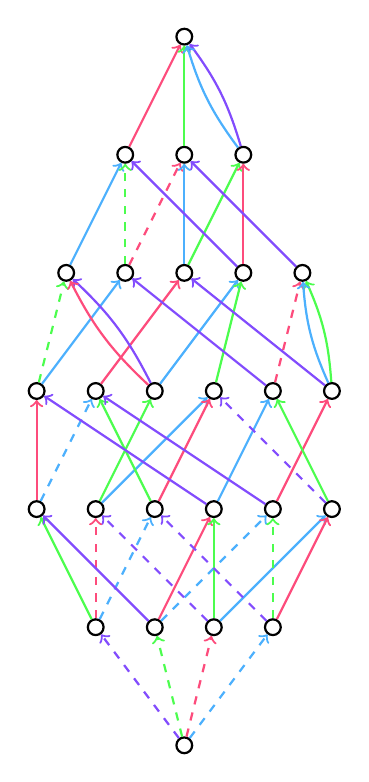
\begin{tikzpicture}[scale=1,bend angle=10]
\newcommand{\xspace}{1}
\newcommand{\yspace}{1}
\tikzstyle{vertex}=[draw,thick,circle,minimum size=2mm,inner sep=0pt]
\tikzstyle{edge}=[thick,->]
\tikzstyle{onesided}=[edge,dashed]
\tikzstyle{bothsided}=[edge]
\tikzstyle{unhighlighted}=[]
\tikzstyle{highlighted}=[]
\definecolor{s1color}{RGB}{130,76,253}
\definecolor{s2color}{RGB}{76,253,78}
\definecolor{s3color}{RGB}{253,76,124}
\definecolor{s4color}{RGB}{76,176,253}
\tikzstyle{s1}=[s1color]
\tikzstyle{s2}=[s2color]
\tikzstyle{s3}=[s3color]
\tikzstyle{s4}=[s4color]
\node[vertex,unhighlighted] (0) at (\xspace*0,\yspace*0) {};
\node[vertex,unhighlighted] (1) at (\xspace*-1.125,\yspace*1.5) {};
\node[vertex,unhighlighted] (2) at (\xspace*-0.375,\yspace*1.5) {};
\node[vertex,unhighlighted] (3) at (\xspace*0.375,\yspace*1.5) {};
\node[vertex,unhighlighted] (4) at (\xspace*1.125,\yspace*1.5) {};
\node[vertex,unhighlighted] (5) at (\xspace*-1.875,\yspace*3) {};
\node[vertex,unhighlighted] (6) at (\xspace*-1.125,\yspace*3) {};
\node[vertex,unhighlighted] (7) at (\xspace*-0.375,\yspace*3) {};
\node[vertex,unhighlighted] (8) at (\xspace*0.375,\yspace*3) {};
\node[vertex,unhighlighted] (9) at (\xspace*1.125,\yspace*3) {};
\node[vertex,unhighlighted] (10) at (\xspace*1.875,\yspace*3) {};
\node[vertex,unhighlighted] (11) at (\xspace*-1.875,\yspace*4.5) {};
\node[vertex,unhighlighted] (12) at (\xspace*-1.125,\yspace*4.5) {};
\node[vertex,unhighlighted] (13) at (\xspace*-0.375,\yspace*4.5) {};
\node[vertex,unhighlighted] (14) at (\xspace*0.375,\yspace*4.5) {};
\node[vertex,unhighlighted] (15) at (\xspace*1.125,\yspace*4.5) {};
\node[vertex,unhighlighted] (16) at (\xspace*1.875,\yspace*4.5) {};
\node[vertex,unhighlighted] (17) at (\xspace*-1.5,\yspace*6) {};
\node[vertex,unhighlighted] (18) at (\xspace*-0.75,\yspace*6) {};
\node[vertex,unhighlighted] (19) at (\xspace*0,\yspace*6) {};
\node[vertex,unhighlighted] (20) at (\xspace*0.75,\yspace*6) {};
\node[vertex,unhighlighted] (21) at (\xspace*1.5,\yspace*6) {};
\node[vertex,unhighlighted] (22) at (\xspace*-0.75,\yspace*7.5) {};
\node[vertex,unhighlighted] (23) at (\xspace*0,\yspace*7.5) {};
\node[vertex,unhighlighted] (24) at (\xspace*0.75,\yspace*7.5) {};
\node[vertex,unhighlighted] (25) at (\xspace*0,\yspace*9) {};
\draw[s1,onesided,unhighlighted] (0) edge (1);
\draw[s2,onesided,unhighlighted] (0) edge (2);
\draw[s3,onesided,unhighlighted] (0) edge (3);
\draw[s4,onesided,unhighlighted] (0) edge (4);
\draw[s2,bothsided,unhighlighted] (1) edge (5);
\draw[s3,onesided,unhighlighted] (1) edge (6);
\draw[s4,onesided,unhighlighted] (1) edge (7);
\draw[s1,bothsided,unhighlighted] (2) edge (5);
\draw[s3,bothsided,unhighlighted] (2) edge (8);
\draw[s4,onesided,unhighlighted] (2) edge (9);
\draw[s1,onesided,unhighlighted] (3) edge (6);
\draw[s2,bothsided,unhighlighted] (3) edge (8);
\draw[s4,bothsided,unhighlighted] (3) edge (10);
\draw[s1,onesided,unhighlighted] (4) edge (7);
\draw[s2,onesided,unhighlighted] (4) edge (9);
\draw[s3,bothsided,unhighlighted] (4) edge (10);
\draw[s3,bothsided,unhighlighted] (5) edge (11);
\draw[s4,onesided,unhighlighted] (5) edge (12);
\draw[s2,bothsided,unhighlighted] (6) edge (13);
\draw[s4,bothsided,unhighlighted] (6) edge (14);
\draw[s2,bothsided,unhighlighted] (7) edge (12);
\draw[s3,bothsided,unhighlighted] (7) edge (14);
\draw[s1,bothsided,unhighlighted] (8) edge (11);
\draw[s4,bothsided,unhighlighted] (8) edge (15);
\draw[s1,bothsided,unhighlighted] (9) edge (12);
\draw[s3,bothsided,unhighlighted] (9) edge (16);
\draw[s1,onesided,unhighlighted] (10) edge (14);
\draw[s2,bothsided,unhighlighted] (10) edge (15);
\draw[s2,onesided,unhighlighted] (11) edge (17);
\draw[s4,bothsided,unhighlighted] (11) edge (18);
\draw[s3,bothsided,unhighlighted] (12) edge (19);
\draw[s1,bothsided,unhighlighted,bend right] (13) edge (17);
\draw[s3,bothsided,unhighlighted,bend left] (13) edge (17);
\draw[s4,bothsided,unhighlighted] (13) edge (20);
\draw[s2,bothsided,unhighlighted] (14) edge (20);
\draw[s1,bothsided,unhighlighted] (15) edge (18);
\draw[s3,onesided,unhighlighted] (15) edge (21);
\draw[s1,bothsided,unhighlighted] (16) edge (19);
\draw[s2,bothsided,unhighlighted,bend right] (16) edge (21);
\draw[s4,bothsided,unhighlighted,bend left] (16) edge (21);
\draw[s4,bothsided,unhighlighted] (17) edge (22);
\draw[s2,onesided,unhighlighted] (18) edge (22);
\draw[s3,onesided,unhighlighted] (18) edge (23);
\draw[s4,bothsided,unhighlighted] (19) edge (23);
\draw[s2,bothsided,unhighlighted] (19) edge (24);
\draw[s1,bothsided,unhighlighted] (20) edge (22);
\draw[s3,bothsided,unhighlighted] (20) edge (24);
\draw[s1,bothsided,unhighlighted] (21) edge (23);
\draw[s3,bothsided,unhighlighted] (22) edge (25);
\draw[s2,bothsided,unhighlighted] (23) edge (25);
\draw[s1,bothsided,unhighlighted,bend right] (24) edge (25);
\draw[s4,bothsided,unhighlighted,bend left] (24) edge (25);
\end{tikzpicture}
		\caption{Hasse diagram of $Wk(A_4, \id)$}
		\label{fig:a4}
	\end{figure}
\end{exam}

\begin{lemm}
	\typedlabel{lemm:wk-subposet-of-br}
	The poset $Wk(\theta)$ is a subposet of $\Br(\ti{\theta})$.

	\begin{proof}
		Both posets are defined on $\ti{\theta}$. Let $w,v \in \ti{\theta}$ be two twisted involutions. Assume $w \preceq v$ with $w \ul s = v$ for some $s \in S$. If $\ul s$ acts by multiplication on $w$, then $ws = v$ and since $s \in T$ ($T$ the set of all reflections in $W$) and $l(w \ul s) = l(w) + 1$ we have $w \leq v$. If conversely $\ul s$ acts by twisted conjugation on $w$, then $v = \theta(s)ws = w (w^{-1} \theta(s) w)(e^{-1}se)$ and since $w^{-1} \theta(s) w, s \in T$ and $l(w \ul s) = l(\theta(s)w) + 1 = l(w) + 2$ we have again $w \leq v$.
	\end{proof}
\end{lemm}

\begin{prop}
	\typedlabel{prop:w-ul-s-leq-w-iff-s-in-dr-w}
	For all $w \in \ti{\theta}$ and $s \in S$ we have $w \ul s \prec w$ iff $s \in D_R(w)$ and $w \ul s \succ w$ iff $s \notin D_R(w)$ as well as $w \ul s < w$ iff $s \in D_R(w)$ and $w \ul s > w$ iff $s \notin D_R(w)$.

	\begin{proof}
		We have $w \ul s \ul s = w$ and $\rho(w \ul s) = \rho(w) - 1$ iff $s \in D_R(w)$ and $\rho(w \ul s) = \rho(w) + 1$ iff $s \notin D_R(w)$ by \ref{lemm:rho-w-ul-s-minus-rho-w-differs-by-1}. By \ref{lemm:wk-subposet-of-br} both statements are true for $\Br(\ti{\theta})$, too.
	\end{proof}
\end{prop}

\begin{defi}
	Let $v,w \in W$ with $\rho(w) - \rho(v) = n$. A sequence $v = w_0 \prec w_1 \prec \ldots \prec w_n = w$ is called a \defword{geodesic} from $v$ to $w$.
\end{defi}

\begin{prop}
	\typedlabel{prop:geodesics-have-same-count-of-multiplicative-steps}
	Let $v,w \in W$ with $v \prec w$. Then all geodesics from $v$ to $w$ have the same count of twisted conjugated and multiplicative steps.

	\begin{proof}
		Suppose we have two geodesics from $v$ to $w$, where the first has $n$ and the second $m$ multiplicative steps. Then $l(w) + n + 2(k-n) = l(v) = l(w) + m + 2(k-m)$, hence $n = m$.
	\end{proof}
\end{prop}

\begin{lemm}
	\typedlabel{lemm:no-triple-edges}
	Let $w \in W$ and $w \ul s \succ w$. Then $|\{ t \in S : w \ul t = w \ul s \}| \in \{1,2\}$.

	\begin{proof}
		Suppose $t \in S \setminus D_R(w)$ with $w \ul t = w \ul s$. Because of the ordinary length either both $\ul s$ and $\ul t$ act by multiplication on $w$, or both act by twisted conjugation on $w$. Suppose they act by multiplication, then $ws = w \ul s = w \ul t = wt$, hence $s = t$. Conversely, assume they act by twisted conjugation. Then $\theta(s) w s = w \ul s = w \ul t = \theta(t)wt$. Because of $\theta(t) w t t = \theta(t) w = \theta(s) w s t$ we have $l(\theta(s) w s t) < l(\theta(s) w s)$ and so by \ref{coro:exchange-condition} there are three possible cases
		$$ \theta(t)w = \theta(s) w s t = \begin{cases}
			\theta(s) w & \Rightarrow s = t, \\
			w s & \Rightarrow \theta(t) = w s w^{-1} \textrm{ or} \\
			\theta(s) \overline w s & \Rightarrow w = \theta(t) \theta(s) \overline w s, \\
		\end{cases} $$
		where $\overline w$ denotes a well chosen subexpression of $w$. The first case is trivial, the second determines $t$ unambiguously. The third case is impossible, since by \ref{coro:exchange-condition} and \ref{rema:exchange-condition-left-sided} we would have a reduced expression for $w$ beginning with $\theta(s)$ or ending with $s$ (or both), yielding $l(\theta(s)ws) \leq l(w)$, which contradicts to $\rho(w \ul s) = \rho(\theta(s)ws) > \rho(w)$. Therefore, there cannot be more than two distinct $s,t \in S \setminus D_R(w)$ with $w \ul s = w \ul t$.
	\end{proof}
\end{lemm}

\begin{lemm}
	\typedlabel{lemm:double-edges-only-for-ord-2}
	Let $w \in \ti{\theta}$ and $s,t \in S$ be two distinct generators. If $w \ul s = w \ul t$, then $\ord(st) = 2$.

	\begin{proof}
		By the proof of \ref{lemm:no-triple-edges} we see that $w \ul s = w \ul t$ for two distinct $s,t \in S$ implies that $\theta(t)w = ws$ holds and that $\ul s$ and $\ul t$ act by twisted conjugation on $w$. Since $\theta(w) = w^{-1}$ we also have $\theta(s)w = wt$ by
		$$ \theta(t)w = ws \iff \theta(\theta(t)w) = \theta(ws) \iff tw^{-1} = w^{-1} \theta(s) \iff wt = \theta(s)w. $$
		Hence, we have $wts = \theta(s)ws = \theta(t)wt = wst$, yielding $st = ts$ and $\ord(st) = 2$.
	\end{proof}
\end{lemm}